%%%%%%%%%%%%%%%%%%%%%%%%%%%%%%%%%%%%%%%%%
% Beamer Presentation
% LaTeX Template
% Version 1.0 (10/11/12)
%
% This template has been downloaded from:
% http://www.LaTeXTemplates.com
%
% License:
% CC BY-NC-SA 3.0 (http://creativecommons.org/licenses/by-nc-sa/3.0/)
%
%%%%%%%%%%%%%%%%%%%%%%%%%%%%%%%%%%%%%%%%%

%----------------------------------------------------------------------------------------
%	PACKAGES AND THEMES
%----------------------------------------------------------------------------------------
\documentclass[aspectratio=43,UTF8,10pt,t]{ctexbeamer}

\mode<presentation> {
\usetheme{Madrid}
\setbeamertemplate{footline}[frame number] % To remove the footer line in all slides
\setbeamercolor{page number in head/foot}{fg=blue}
\setbeamertemplate{navigation symbols}{} % To remove the navigation symbols from the bottom of all slides
}

% User Defined Block %%%%%%%%%%%%%%%%%%%%%%%%%%%%%%%%%%%%%%%%%%%%%%%%%%%%%%%%
\usepackage{setspace}
\definecolor{hanblue}{rgb}{0.27, 0.42, 0.81}
\definecolor{indiagreen}{rgb}{0.07, 0.53, 0.03}
\definecolor{indianred}{rgb}{0.8, 0.36, 0.36}
\definecolor{indianyellow}{rgb}{0.89, 0.66, 0.34}
\definecolor{babypink}{rgb}{0.96, 0.76, 0.76}
\definecolor{ao(english)}{rgb}{0.0, 0.5, 0.0}
\setbeamerfont{block title}{size=\normalsize}
\setbeamerfont{block body}{size=\small}
\newenvironment<>{blueblock}[1]{%
  \setbeamercolor{block title}{fg=white,bg=hanblue}%
  \begin{block}#2{#1}}{\end{block}}
\newenvironment<>{greenblock}[1]{%
  \setstretch{1.3}\setbeamercolor{block title}{fg=white,bg=indiagreen}%
  \begin{block}#2{#1}}{\end{block}}
\newenvironment<>{redblock}[1]{%
  \setstretch{1.3}\setbeamercolor{block title}{fg=white,bg=indianred}%
  \begin{block}#2{#1}}{\end{block}}
\newenvironment<>{yellowblock}[1]{%
  \setstretch{1.3}\setbeamercolor{block title}{fg=white,bg=indianyellow}%
  \begin{block}#2{#1}}{\end{block}}

%----------------------------------------------------------------------------------------
%	PACKAGES
%----------------------------------------------------------------------------------------
\usepackage{graphicx} % Allows including images
%\usepackage{tikz}
%\usetikzlibrary{shapes.geometric, arrows}
\usepackage{float}
\usepackage{listings}
\usepackage{multicol}
\usepackage{ctex}
\lstset{language=C++,
    columns=flexible,
    basicstyle=\footnotesize\ttfamily,                                      % 设定代码字体、大小
    %numbers=left,xleftmargin=2em,framexleftmargin=2em,                   % 在左侧显示行号
    %numberstyle=\color{darkgray},                                        % 设定行号格式
    keywordstyle=\color{blue},                                            % 设定关键字格式
    commentstyle=\color{ao(english)},                                     % 设置代码注释的格式
    stringstyle=\color{brown},                                            % 设置字符串格式
    %showstringspaces=false,                                              % 控制是否显示空格
	%frame=lines,                                                         % 控制外框
    breaklines,                                                           % 控制是否折行
    postbreak=\space,                                                     % 控制折行后显示的标识字符
    breakindent=5pt,                                                      % 控制折行后缩进数量
    emph={size\_t,array,deque,list,map,queue,set,stack,vector,string,pair,tuple}, % 非内置类型
    emphstyle={\color{teal}},
    escapeinside={(*@}{@*)},
}

%----------------------------------------------------------------------------------------
%	TITLE PAGE
%----------------------------------------------------------------------------------------

\title[\textit{C++程序设计:第七章}]{第七章~模板与泛型编程} % The short title appears at the bottom of every slide, the full title is only on the title page

%\author[李长河]{李长河} % Your name
%\institute[CUG] % Your institution as it will appear on the bottom of every slide, may be shorthand to save space
%{
%中国地质大学(武汉)\\ % Your institution for the title page
%\medskip
%\textit{lichanghe@cug.edu.cn} % Your email address
%}
%\date{} % Date, can be changed to a custom date

\begin{document}

%----------------------------------------------------------------------------------------
%	TIKZ FLOWCHART
%----------------------------------------------------------------------------------------
%\tikzstyle{startstop} = [rectangle, rounded corners, minimum width=2cm, minimum height=0.5cm, text centered, draw=black, fill=red!30, font=\tiny]
%\tikzstyle{io} = [trapezium, trapezium left angle=70, trapezium right angle=110, minimum width=0cm, minimum height=0cm, text centered, draw=black, fill=blue!30, font=\tiny]
%\tikzstyle{process} = [rectangle, minimum width=2.5cm, minimum height=1.5cm, text centered, draw=black, fill=orange!30, font=\tiny, text width=2cm]
%\tikzstyle{decision} = [diamond, minimum width=2.5cm, minimum height=2cm, text centered, draw=black, fill=green!30, font=\tiny, text width=1.8cm, aspect=1.1]

\begin{frame}[fragile]{7.3.1快速排序}
\tableofcontents
\end{frame}
\begin{frame}[fragile]{7.3.1快速排序}
\section{快速排序的定义和优点}
\begin{block}{1 快速排序的定义和优点}
  快速排序是冒泡排序的改进,在排序过程中数据移动少,是目前已知的最快的排序方法。\\
\end{block}
\section{快速排序的基本思想}
\begin{block}{2 快速排序的基本思想}
基本思想:划分和分治递归。\\
   第一步划分:将整个数组划分为两个部分,第一部分所有值小于基准值(key),第二部分所以值大于基准值(key)。基准值的选择是随机的,(一般选择待排数组的第一个元素)。\\
   第二步分治递归:第一步将数组划分为两部分后,两部分内部还不是有序的,再分别对两部分递归地进行快速排序,最终得到一个完整的有序数组。\\
\end{block}
\end{frame}

\begin{frame}[fragile]{7.3.1 快速排序}
\section{快速排序的流程}
\begin{block}{3 快速排序的流程}
(1)left、right指针(索引)分别指向待排数组的首、尾。\\
(2)left 指针向后遍历,right指针向前遍历。\\
(3)当right指针指向元素小于基准值(key)时,right指针元素便赋值给left指针元素,完成转移。\\
(4)当left指针指向元素大于基准值(key)时,left指针元素便赋值给right指针元素,完成转移。\\
(5)最终当left=right时,遍历结束。\\
(6)以基准值(key)为界限,把数组分成两部分,分别对这两部分进行快速排序(显然这是一个递归的过程)\\
\end{block}
\end{frame}
\begin{frame}[fragile]{7.3.1 快速排序}
\begin{block}{4 快速排序的举例}
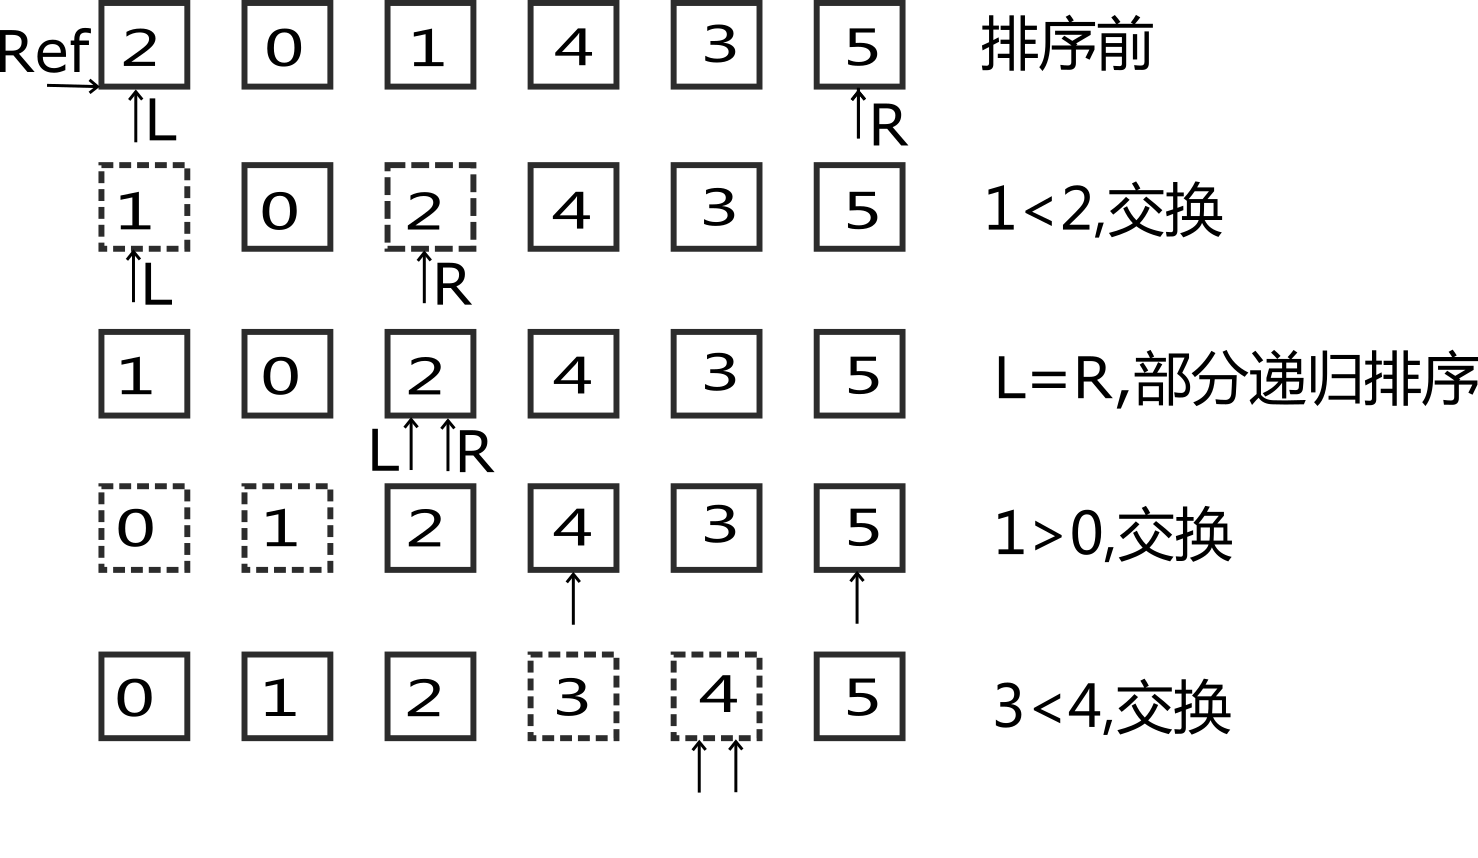
\includegraphics[scale=0.45]{quick_sort.png}
\end{block}
\end{frame}
\begin{frame}[fragile]{7.3.1 快速排序}
\section{快速排序的小技巧}
\begin{block}{5 快速排序的小技巧}
(1)若以数组的第一个元素为基准值,则应该先用right向左遍历,然后再用left向右遍历。\\
~\\
(2)若以数组的最后一个元素为基准值,则应该先用left向右遍历,然后再用right向左遍历。\\
~\\
(3)一般不建议用数组中间的元素做基准值,但也可以用。\\
~\\
\end{block}
\end{frame}

\begin{frame}[fragile]{7.3.1 快速排序}
\section{快速排序的源代码}
\begin{block}{6 快速排序的源代码}
\begin{lstlisting}
template<typename T,size_t N>
void array<T,N>::quicksort(T a[],int left,int right)
{
  if (right <left)
  cout<<" 输入错误";
  else if(right-left==1)
   {
   if (a[left] > a[right])
   swap(a[left], a[right]);
   }
  else
   {T key = a[left];int i = left;int j = right;
    while (i != j)
      { while (i < j && a[j] >= key)  j--;
        while (i < j && a[i] <= key)  i++;
        if (i < j)  swap(a[j], a[i]); }
            a[left] = a[j]; a[i] = key;
     quicksort(a, left, i - 1);//递归调用快速排序
     quicksort(a, i + 1, right);//递归调用快速排序
   }
}
\end{lstlisting}
\end{block}
\end{frame}

\begin{frame}[fragile]{7.3.1快速排序}
\section{课堂小测试}
\begin{block}{7 课堂小测试}
对下列序列进行快速排序,都以第一个元素为基准进行第一次划分,则在该次划分过程中,需要移动元素次数最多的序列是()\\
(A) 1,3,5,7,9  (B)9,7,5,3,1\\
(c) 5,1,3,7,9  (D)5,7,9,3,1\\
\includegraphics[scale=0.3]{quick_sort_1.jpg}
\end{block}
\end{frame}
\end{document} 